% 原书印刷162--175／PDF物理187--200.
\subsubsection{分支运输}\label{sec:4.4.2}\index{B017@分支传输（branched transport）|hyperpage}\index{N107@网络（networks）!109@分支（ramified）|hyperpage}

\phantomsection\label{idx:root4-p162-subadditivity}\index{S145@次可加性（sub-additivity）|hyperpage}“讨论”部分的第二部分旨在介绍一个相反的最小流问题：与交通拥挤的情形不同，这里鼓励沿同一路径共同运输. 考虑“规模经济”原则时，这是合理的，也能在许多不同现象中观察到. 在许多情形中，当一个规划者需要组织运输（例如建设运输网络）时，总成本具有\emph{次可加性}：移动两个对象的成本不超过分别移动它们的两个成本之和；而且在许多情形中具有\emph{递减边际成本}，即在给定背景数量上增加一个单位的成本，是背景数量的递减函数，这意味着成本实际上为凹函数.

注意，此处将运输成本视为质量的函数，而非长度的函数. 隐含假设是，成本关于长度线性，如同本章全部最小流问题一样；但它关于质量为凹，与\autoref{sec:3.3.2}中所见相反.

许多运输不同流体的分支结构，例如道路系统、通信网络、河流流域、血管、树叶、树木等，都很容易被理解为这类成本的变分原理所产生的结果.

还要注意，恰如交通拥挤的情形，无论使用Lagrange语言还是Euler语言，为这类效应建模都需要考察每个粒子实际经过的路径，不能仅使用一个运输方案$\gamma\in\Pi(\mu,\nu)$完成. 不过，一旦利用本章发展的工具选定合适表述，就可以猜测这类问题最优解的形状：粒子在某些点汇集，尽可能共同运动，然后分支前往不同目的地. 因而这类问题如今被称为“分支运输”（branched transport）.

近来，这些问题受到了数学家的广泛关注；但事实上，可以用Dirac质量表达的离散框架的形式化，在优化与运筹学中早已十分经典. 与拥挤运输一样，先从Gilbert引入的离散框架\cite{b185}开始. 然后转向更新近的连续模型：Lagrange模型的一部分由Bernot、Caselles与Morel\cite{b46,b48,b49,b50}以及Maddalena与Solimini\cite{b220,b221}发展和研究；Xia\cite{b297}则给出了Gilbert能量的Euler连续推广.

\paragraph{离散模型}
用本章语言改述Gilbert的工作\cite{b185}，考虑支于某个紧子集$\Omega\subset\mathbb R^d$上的两个原子概率测度$\mu=\sum_{i=1}^m a_i\delta_{x_i}$和$\nu=\sum_{j=1}^n b_j\delta_{y_j}$，希望通过一个加权有向图$G$连接它们. $\mathbb R^d$中的\emph{加权有向图}是一个系统$G=(s_k,\theta_k)_k$，其中$s_k=(p_k,q_k)$是一对点，表示$\mathbb R^d$中的有向线段，$\theta_k\in\mathbb R_+$是与线段$s_k$关联的权重. 用$\hat s_k$表示$s_k$的方向$(q_k-p_k)/|q_k-p_k|$（假设线段非退化），用$|s_k|$表示其长度$|q_k-p_k|$. 点$p_k,q_k$称为图的\emph{顶点}，线段$s_k$称为图的\emph{边}.

\begin{center}
 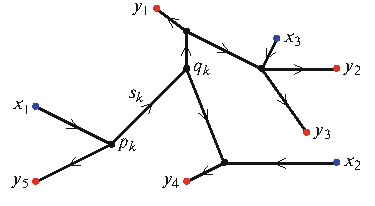
\includegraphics[width=.58\textwidth]{assets/ch04c-unnum-graph.pdf}
\end{center}

给定$\mu,\nu$，若$G$满足电路中众所周知的Kirchhoff定律，即对图的每个顶点$x$都有
\[
 x\text{处的流入质量}=x\text{处的流出质量},
\]
则称$G$从$\mu$灌溉$\nu$. 流入质量包括到达$x$的线段$s_k=(p_k,q_k)$（即$x=q_k$）所携带的质量，再加上$\mu$给出的质量，即$x=x_i$时再加$a_i$. 类似地，$x$处的流出质量是离开$x$的线段$s_k=(p_k,q_k)$（即$p_k=x$）的总权重，减去$\nu$取走的质量，即$x=y_j$时减去$b_j$. 从$\mu$灌溉$\nu$的图的集合记为$\mathrm G(\mu,\nu)$.

对$\alpha\in[0,1]$，定义图$G$的$\alpha$-灌溉成本，又称Gilbert能量，为
\[
 \mathscr E_\alpha(G)=\sum_{k=1}^n\theta_k^\alpha|s_k|,
\]
这意味着，将质量$m$沿长度为$l$的线段移动的成本是$m^\alpha l$.

给定原子概率$\mu,\nu$，希望在所有将$\mu$送至$\nu$的图中极小化该能量，即
\[
 \min\{\mathscr E_\alpha(G):G\in\mathrm G(\mu,\nu)\}.
\]
\phantomsection\label{idx:root4-p163-steiner}\index{S143@Steiner问题（Steiner problem）|hyperpage}Gilbert在\cite{b185,b186}中引入这一问题，将其作为Steiner最小长度问题的推广；后者对应于\footnote{要使Steiner最小连接问题与$\alpha=0$的Gilbert问题严格等价，需要考虑由单个Dirac质量组成的测度$\mu$，这样$\operatorname{spt}(\nu)$中的每个点都必须与它连接，从而保证图连通.}$\alpha=0$的情形，其目标是极小化网络总长度. Gilbert所提及的主要应用属于通信网络领域.

注意，对$\alpha\in[0,1]$，函数$t\mapsto t^\alpha$为凹且次可加；对$\alpha\in(0,1)$，它严格凹. 因此，比起使用若干较小管道运输相同总质量，更倾向于使用将质量从$\mu$送至$\nu$的较大管道.

\begin{figure}[htbp]
 \centering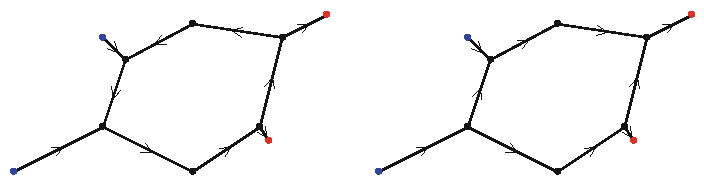
\includegraphics[width=.9\textwidth]{assets/ch04c-fig4-5.pdf}
 \caption{一个强环的例子（左），以及一个不是强环的环（右）.}
 \label{fig:4.5}
\end{figure}

这个问题为何存在极小解，并不显然. 事实上，我们在有限对象中极小化，却没有对边数、顶点数等施加一致界. 需要给出一个重要定义.\footnote{遗憾的是，为遵从分支运输中通常采用的语言，不能与本章其余部分完全一致；此前所称的“环流”，在这里称为“强环”.}

\begin{definition}\label{obj:4.37}\index{C035@环（cycles）|hyperpage}
将$G$中任意一列相邻的线段（相应地，有向线段）称为\emph{环}（相应地，\emph{强环}），见\autoref{fig:4.5}.
\end{definition}

由于$t\mapsto t^\alpha$递增，通过去掉强环就容易降低图的能量. 不难验证，同一函数的凹性还保证，去掉任意环都能降低能量. 因此可以取一列无环、即为树的图作为极小化序列，这使边数具有一致上界，其界由$\mu$与$\nu$的原子总数给出. 由此得到紧性，并证明极小解存在. 任意极小解都没有强环；当$\alpha\in(0,1)$时，也没有环.

此外，可以证明图中自由接合点的一个最优性条件. 也就是说，对图中每个不属于$x_i$或$y_j$的节点$x$，必须满足方向平衡条件：
\begin{equation}\label{eq:4.31}\index{A009@角度定律（angle laws）|hyperpage}
 \sum_{k:x=p_k}\theta_k^\alpha\hat s_k
 -\sum_{k:x=q_k}\theta_k^\alpha\hat s_k=0.
\end{equation}

这意味着，所有接触点$x$的线段对应的单位向量之和必须为零；这些向量一律取为从$x$出发，而不管真实方向$\hat s_k$，并各自乘上权重$\theta_k^\alpha$.\footnote{对于最常见的三重接合点，这给出有趣的结果：$\alpha=0$时得到Steiner树众所周知的三个角均为$120^\circ$的条件，$\alpha=0.5$时得到一个$90^\circ$角，见\autoref{ex:30}；不过，一般而言，角度依赖于质量$\theta_k$.}

\paragraph{Xia的松弛连续模型}
Xia在较近的工作\cite{b297}中提出一种新形式化，将这一问题推广到任意概率测度$\mu,\nu$. 主要思路是将Kirchhoff定律约束变为散度约束. 为准确表述，并且由于后面需要使用这种语言，先引入一些较繁复的记号.

\phantomsection\label{idx:root4-p165-rectifiability}\index{R127@可求长性（rectifiability）!128@分支网络（branched networks）|hyperpage}若$E\subset\Omega$是1-可求长集，\footnote{研究凸函数可微性时，已在\autoref{sec:1}遇到可求长集：1-可求长集定义为在$\mathscr H^1$-几乎处处意义下被可数条Lipschitz曲线的并覆盖的集合. 无论如何，读者可以暂把“1-可求长”理解为“一维”的同义词，这已足以理解余下讨论.}$\tau:E\to\mathbb S^{d-1}$是可测向量场，$\theta:E\to\mathbb R_+$关于$\mathscr H^1$可积，则对所有$\xi\in C(\Omega;\mathbb R^d)$，通过
\[
 \langle[E,\tau,\theta],\xi\rangle
 =\int_E\theta(x)\xi(x)\cdot\tau(x)\,\mathrm d\mathscr H^1(x)
\]
定义有限向量测度$[E,\tau,\theta]\in\mathscr M^d(\Omega)$.

给定有限图$G=(s_k,\theta_k)_k$，为$G$关联测度
\[
 \mathbf w_G:=\sum_k[s_k,\hat s_k,\theta_k]\in\mathscr M^d(\Omega).
\]
成本和约束均可只用$\mathbf w_G$表达. 首先注意，$G\in\mathrm G(\mu,\nu)$（即满足从$\mu$灌溉$\nu$的质量平衡条件），当且仅当$\nabla\cdot\mathbf w_G=\mu-\nu$. 此外，有
\[
 \mathscr E_\alpha(G)=\sum_{k=1}^n\theta_k^\alpha|s_k|
                  =\int_K|\theta(x)|^\alpha\,\mathrm d\mathscr H^1(x),
\]
其中$\theta$表示$\mathbf w_G$关于$\mathscr H^1$测度的密度.

这提示了通过推广Gilbert能量来建立Gilbert问题的连续Euler表述，极小化问题变为
\begin{equation}\label{eq:4.32}
 (\mathrm{XP})\quad
 \min\{M_\alpha(\mathbf w):\mathbf w\in\mathscr M^d_{\mathrm{div}}(\Omega),
                                \ \nabla\cdot\mathbf w=\mu-\nu\}.
\end{equation}
\phantomsection\label{idx:root4-p165-relaxation}\index{R134@松弛（relaxation）|hyperpage}显然，需要定义能量$M_\alpha$，它也称为$\mathbf w$的“$\alpha$-质量”. Xia原先的思路是通过松弛定义，即
\begin{equation*}
\begin{aligned}
 M_\alpha(\mathbf w):=\inf\bigl\{&\liminf_n\mathscr E_\alpha(G_n):
                  G_n\in\mathrm G(\mu_n,\nu_n),\\
            &\mathbf w_{G_n}\rightharpoonup\mathbf w
                     \text{ 于 }\mathscr M^d_{\mathrm{div}}(\Omega)\bigr\},
\end{aligned}
\end{equation*}
其中在$\mathscr M^d_{\mathrm{div}}(\Omega)$中收敛意味着，作为测度有$\mathbf w_{G_n}\rightharpoonup\mathbf w$以及$\nabla\cdot\mathbf w_{G_n}=\mu_n-\nu_n\rightharpoonup\nabla\cdot\mathbf w$.

\phantomsection\label{idx:root4-p166-rectifiability}\index{R127@可求长性（rectifiability）!128@分支网络（branched networks）|hyperpage}由B.~White的一个著名可求长性定理\cite{b296}，可以证明$M_\alpha(\mathbf w)<+\infty$蕴含$\mathbf w$是1-可求长的；\footnote{将可求长向量测度定义为可写成$[E,\tau,\theta]$形式且$E$可求长的向量测度. 这一语言借自可求长流的语言，但流可视为向量测度. 详见\cite{b161}.}进一步精细分析可得
\[
 M_\alpha(\mathbf w)=\begin{cases}
 \displaystyle\int_E|\theta(x)|^\alpha\,\mathrm d\mathscr H^1(x),
                   &\mathbf w=[E,\tau,\theta],\\
 +\infty,&\text{其他情形}.
 \end{cases}
\]
应证明，当$\mu$与$\nu$都是原子测度时，能够回到Gilbert的问题；这并不平凡，因为已经允许了大量新的竞争者.

与有限原子情形相比，另一个差别是\hyperref[eq:4.32]{(XP)}最小值的有限性. 确实，总可用有限图连接两个原子测度，有限图的成本也总是有限. 但对一般测度$\mu,\nu$，却不清楚是否存在满足$M_\alpha(\mathbf w)<\infty$和$\nabla\cdot\mathbf w=\mu-\nu$的$\mathbf w$.

\paragraph{可灌溉性与灌溉距离}
\phantomsection\label{idx:root4-p166-irrigation-distance}\index{B017@分支传输（branched transport）!018@$d_\alpha$距离（$d_\alpha$ distance）|hyperpage}对$\mu,\nu\in\mathscr P(\Omega)$，令$d_\alpha(\mu,\nu):=\min(\mathrm{XP})\in[0,+\infty]$，它显然依赖于$\mu,\nu$. 首先考察该值是否有限. 假设$0\in\Omega$，显然若$d_\alpha(\mu,\delta_0),d_\alpha(\nu,\delta_0)<+\infty$，则$d_\alpha(\mu,\nu)<+\infty$. 因此，\footnote{事实上，虽然并不完全显然，但可以证明，至少当$\operatorname{spt}(\mu)\cap\operatorname{spt}(\nu)=\varnothing$时，条件$d_\alpha(\mu,\nu)<+\infty$实际上等价于$d_\alpha(\mu,\delta_0),d_\alpha(\nu,\delta_0)<+\infty$.}将专注于$d_\alpha(\mu,\delta_0)<+\infty$是否成立.

\cite{b297}中的一个主要结果如下：
\begin{proposition}\label{obj:4.38}
若$\alpha>1-1/d$且$\Omega=[-a,a]^d$，则对每个$\mu\in\mathscr P(\Omega)$，有$d_\alpha(\mu,\delta_0)<+\infty$. 这蕴含对每对$(\mu,\nu)$均有$d_\alpha(\mu,\nu)<+\infty$. 任意紧区域上也成立，只需将它装入一个大立方体.

此外，仍在$\alpha>1-1/d$及$\Omega$紧的条件下，$d_\alpha$确实是$\mathscr P(\Omega)$上的距离，并且使概率的弱收敛可度量化.
\end{proposition}
这里只证明这一陈述的第一部分.
\begin{proof}
证明$d_\alpha(\mu,\delta_0)<+\infty$的思路如下：将立方体$\Omega$分成$2^{nd}$个边长为$2^{-n}$的小立方体，并在每个小立方体的中心放置质量等于该立方体测度的Dirac质量，得到原子测度$\mu_n$，从而构造$\mu$的二进逼近. 随后通过一个有限图$G_n$（为其关联流$\mathbf w_n$）连接$\mu_n$与$\mu_{n+1}$，将$\mu_n$中对应于小立方体$D$的每个Dirac质量，沿直线送至$\mu_{n+1}$中对应于$D$的子立方体的$2^d$个Dirac质量，见\autoref{fig:4.6}. 简单计算给出估计
\[
 M_\alpha(G_n)\leq C\sum_{k=1}^{2^{nd}}a m_k^\alpha2^{-n},
\]
其中$m_k$是第$n$次分割中各立方体所包含的质量. 随后使用由Jensen不等式得到的$\sum_{k=1}^N m_k^\alpha\leq N^{1-\alpha}(\sum_{k=1}^N m_k)^\alpha$，得到$\mathscr E_\alpha(G_n)\leq aC2^{-n(1-d(1-\alpha))}$.

由构造可知，只需$\sum_n\mathscr E_\alpha(G_n)<+\infty$，而只要$1-d(1-\alpha)>0$，这一条件就成立.
\end{proof}

\begin{figure}[htbp]
 \centering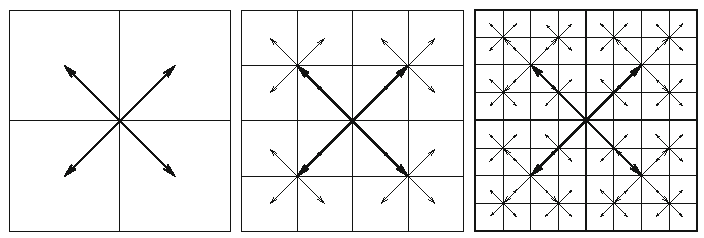
\includegraphics[width=.92\textwidth]{assets/ch04c-fig4-6.pdf}
 \caption{\autoref{obj:4.38}构造的不同步骤.}
 \label{fig:4.6}
\end{figure}

一些反例补充了上述结果，并表明关于$\alpha$的陈述是尖锐的；此处不展开，见\autoref{ex:29}. 更一般地，可以认为从$\delta_0$出发灌溉一个测度的可行性，与它的维数有关；但必须选择适当的维数概念，而不能仅用支集的Hausdorff维数. 这些问题在\cite{b153,b154}中讨论.

有趣的是，上述距离$d_\alpha$也可以通过松弛得到，见\cite{b220}：从一个为每对原子概率测度$\mu=\sum_i a_i\delta_{x_i}$、$\nu=\sum_j b_j\delta_{y_j}$关联量
\[
 \overline d_\alpha(\mu,\nu):=
 \min\left\{\sum_{ij}|x_i-y_j|\gamma(\{(x_i,y_j)\})^\alpha:
                                     \gamma\in\Pi(\mu,\nu)\right\}
\]
的泛函出发. 这一量对应于Kantorovich问题的一种非线性版本，只在原子测度上有良好定义. 随后可以验证
\begin{equation}\label{eq:4.33}
\begin{aligned}
 d_\alpha=\sup\biggl\{&d:\mathscr P(\Omega)\times\mathscr P(\Omega)\to[0,+\infty]:\\
 &\begin{cases}
 d\leq\overline d_\alpha&\text{在原子测度上},\\
 d\text{ 关于弱收敛 }\rightharpoonup\text{ 下半连续},\\
 d\text{ 满足三角不等式}
 \end{cases}\biggr\}.
\end{aligned}
\end{equation}

\paragraph{拉格朗日表述}
现在我们希望给出分支运输问题的另一种表述，它基于路径上的测度. 这一表述\footnote{这里所给出的只是将\cite{b48,b221}提出的模型改写成本章的语言；这些文献使用“参数化交通计划”而非路径上的测度，不过这只是语言上的差别.}由\cite{b221}引入，随后在\cite{b48}中得到深入研究.

\phantomsection\label{idx:root4-p168-traffic-plan}\index{M098@曲线上的测度（measures on curves）|hyperpage}\index{T150@交通方案（traffic plans）|hyperpage}像往常一样，给定两个测度$\mu,\nu\in\mathscr P(\Omega)$，我们寻找一个交通计划\footnote{这一术语正是由\cite{b48}的作者为此目的引入的.}，即测度$Q\in\mathscr P(\mathscr C)$，其中$\mathscr C:=\mathrm{AC}(\Omega)$，且$\int_\mathscr C L(\omega)\,dQ(\omega)<+\infty$. 同样，我们只考虑满足$(e_0)_\#Q=\mu$、$(e_1)_\#Q=\nu$的交通计划（这里不考虑同时固定耦合$(e_0,e_1)_\#Q=\gamma$的情形；顺便指出，若固定$\gamma$，它与前面Xia的欧拉模型之间的联系就不再成立）.

为了引入需要最小化的量，必须先定义
\[
 \theta_Q(x):=Q\bigl(\{\omega\in \mathscr C:x\in\omega([0,1])\}\bigr),\qquad
 m_Q(x):=\int_\mathscr C\#\bigl(\{t\in[0,1]:\omega(t)=x\}\bigr)\,dQ(\omega).
\]
\begin{proposition}\label{obj:4.39}
下列性质成立：
\begin{enumerate}
 \item 总有$0\leq\theta_Q(x)\leq m_Q(x)\leq1$；若$Q$集中在无回路曲线上，则$\theta_Q=m_Q$.
 \item 函数$(x,Q)\mapsto\theta_Q(x)$关于点$x\in\Omega$的收敛及测度$Q\in\mathscr P(\mathscr C)$的弱收敛是上半连续的.
 \item 若存在关于$\mathscr H^1$测度$\sigma$有限的集合$\Gamma$，使得对$Q$几乎处处的曲线$\omega$及几乎处处的时刻$t$，有$\omega(t)\in\Gamma$，则交通强度$i_Q$等于$m_Q\cdot\mathscr H^1$.
\end{enumerate}
\end{proposition}
随后，通过
\[
 I_\alpha(Q):=\int_\mathscr C Z_Q(\omega)\,dQ(\omega)
\]
定义能量$I_\alpha$，其中
\[
 Z_Q(\omega):=L_{\theta_Q^{\alpha-1}}(\omega)
   =\int_0^1\theta_Q(\omega(t))^{\alpha-1}|\omega'(t)|\,dt.
\]
因此，我们考虑的问题是
\[
 \min\{I_\alpha(Q):Q\in\mathscr P(\mathscr C),\ (e_0)_\#Q=\mu,\ (e_1)_\#Q=\nu\}.
\]
注意，平凡的估计$I_\alpha(Q)\geq\int_\mathscr C L(\omega)\,dQ(\omega)$给出了极小化序列的紧性（事实上，能量在每条曲线的重新参数化下不变，因而长度界可转化为Lipschitz界，正如本章其余部分所做的那样）. 接着，通过证明半连续性，便可得到极小元的存在性. 事实上，将性质2与一个简单的Fatou引理结合，得到函数$(Q,\omega)\mapsto Z_Q(\omega)$是下半连续的（$Q$取弱收敛，$\omega$取一致收敛）. 最后使用如下命题：
\begin{proposition}\label{obj:4.40}
若$f:\mathscr P(\mathscr C)\times \mathscr C\to\mathbb R$是下半连续的，则$F:Q\mapsto\int_\mathscr C f(Q,\omega)\,dQ(\omega)$在$\mathscr P(\mathscr C)$上是下半连续的.
\end{proposition}
随后可以证明下列事实：
\begin{proposition}\leavevmode\label{obj:4.41}
\begin{enumerate}
 \item 对每个满足$I_\alpha(Q)<+\infty$的$Q$，集合$\Gamma=\{x:\theta_Q(x)>0\}$关于测度$\mathscr H^1$是$\sigma$有限的，且
 \[
 I_\alpha(Q)=\int_\Gamma\theta_Q^{\alpha-1}m_Q\,d\mathscr H^1.
 \]
 \item 若$Q$最优，则它集中在无回路曲线上，且$I_\alpha(Q)=\int_\Gamma\theta_Q^\alpha\,d\mathscr H^1$.
 \item 若$Q$最优，则它无循环\footnote{可以如下给出精确定义：对$x,y\in\Omega$，定义$[x,y]=\{\omega\in \mathscr C:\exists s<t\text{ 使得 }\omega(s)=x\text{ 且 }\omega(t)=y\}$；若不存在满足$x_1=x_n$的$x_1,\ldots,x_n$，使得对所有$i=1,\ldots,n-1$，都有$Q([x_i,x_{i+1}])>0$或$Q([x_{i+1},x_i])>0$，就称$Q$无循环.}.
\end{enumerate}
\end{proposition}
这一性质，特别是将$I_\alpha$表示为重数$\theta_Q$的$\alpha$次幂之积分的表达式，提示了它与欧拉模型的联系. 可以通过\cite{b48}中的工具，或通过\autoref{obj:4.10}，证明精确的等价性.

\paragraph{单源情形}
当把源测度固定为单个Dirac质量$\delta_0$时，考察问题的特殊性质很有意义. 这一特例本身已经十分丰富. 此时，可以采用另一种重数定义来研究问题：事实上，我们可以预期，只要两条曲线经过同一点$x$，它们在从$0$到$x$的整条路径上就一直同行. 在这种情况下，最好稍微改变一下框架，因为将所有曲线都参数化在某个固定的有限长度区间$[0,1]$上，可能过于受限. 此举也给了我们考察\cite{b221}所提出的原始框架的机会（可以验证它与一般框架等价）.

现在考虑空间$\Lambda=\{\omega\in\operatorname{Lip}_1(\mathbb R_+;\Omega):\omega(0)=0\}$，赋予它紧集上一致收敛的拓扑（回顾这一拓扑可以由某个距离$d$度量化，并且由Ascoli--Arzelà定理，$\Lambda$成为一个紧度量空间）.

若$\omega\in\Lambda$，定义其停止时刻为
\[
 \operatorname{Stop}(\omega)=\inf\{t\geq0:\omega\text{ 在 }[t,+\infty[\text{ 上为常值}\}.
\]
以$\Lambda_{\mathrm{stop}}$表示满足$\operatorname{Stop}(\omega)<\infty$的曲线$\omega$的集合. 随后定义$\Lambda_{\mathrm{stop}}$的下列子集：$\Lambda_{\mathrm{arc}}$、$\Lambda_{\mathrm{inj}}$、$\Lambda_{\mathrm{lf}}$，它们分别由在$[0,\operatorname{Stop}(\omega)]$上按弧长参数化的曲线、在$[0,\operatorname{Stop}(\omega)[$上单射的曲线，以及在$[0,\operatorname{Stop}(\omega)]$上单射的曲线组成（后一类曲线称为无回路曲线）.

将满足
\[
 \int_\Lambda\operatorname{Stop}(\omega)\,d\eta(\omega)<+\infty
\]
的任意$\eta\in\mathscr P(\Lambda)$称为交通模式（使用记号$\eta$，以区别于$Q\in\mathscr P(\mathscr C)$的情形）.

我们用前面定义的如下变体定义重数与能量：对于重数，先定义
\[
 [\omega]_t:=\{\widetilde\omega\in\Lambda_{\mathrm{stop}}:
       \omega(s)=\widetilde\omega(s)\quad\forall s\in[0,t]\},
\]
即直至时刻$t$都与$\omega$重合的曲线的集合；为简化记号，令$|\omega|_{t,\eta}:=\eta([\omega]_t)$. 后一个量将起到重数$\theta$的作用. 随后定义
\[
 \widetilde Z_\eta(\omega):=\int_0^{\operatorname{Stop}(\omega)}
                   |\omega|_{t,\eta}^{\alpha-1}\,dt,
\]
并将满足$\widetilde Z_\eta(\omega)<\infty$的任意曲线$\omega$称为$\eta$良曲线. 然后使用能量
\[
 \widetilde I_\alpha(\eta):=\int_\Lambda\widetilde Z_\eta(\omega)\,d\eta(\omega).
\]
问题变成在满足$(e_\infty)_\#\eta=\nu$的概率测度$\eta\in\mathscr P(\Lambda)$中最小化$\widetilde I_\alpha$，其中$e_\infty(\omega)=\omega(\operatorname{Stop}(\omega))$. 注意，$e_\infty$在$\Lambda_{\mathrm{stop}}$上有良好定义，而任何有限能量交通计划都必然集中在$\Lambda_{\mathrm{stop}}$上，因此这一条件有意义；此外，当限制在任意集合$\{\eta\in\mathscr P(\Lambda):\int_\Lambda\operatorname{Stop}(\omega)\,d\eta(\omega)\leq C\}$上时，$\eta\mapsto(e_\infty)_\#\eta$关于弱收敛连续.

在这种情形下，不难证明极小元的存在性；也可以证明，极小元集中在$\Lambda_{\mathrm{arc}}\cap\Lambda_{\mathrm{inj}}$上，甚至是无回路的（即可以证明$\eta(\Lambda_{\mathrm{lf}})=1$，尽管这不那么显然）. 注意，我们在能量定义中去掉了$|\omega'|$这一项，这迫使极小元使约束$|\omega'|\leq1$饱和.
\begin{remark}\label{obj:4.42}
还可以引入其他介于其间的模型，它们之间的区别都在于曲线$\omega$在时刻$t$的重数定义. 例如见\cite{b47}或\cite{b220}.
\end{remark}
$\eta$良曲线类是一个显式定义的曲线集合，具有许多在$\eta$几乎处处成立的性质. 例如，若$\eta$最优，而$Q$是在适当的时间重新参数化后代表$\eta$的$\mathscr C$上的测度，则有$|\omega|_{t,\eta}=\theta_Q(\omega(t))=m_Q(\omega(t))$，而且对每条$\eta$良曲线$\omega$都成立.

一个重要事实如下：若$\omega_1,\omega_2$是$\eta$良曲线，$\eta$最优，且$(e_\infty)(\omega_1)=(e_\infty)(\omega_2)$，则$\widetilde Z_\eta(\omega_1)=\widetilde Z_\eta(\omega_2)$（见\cite{b272}）. 由此得到的推论之一是，任何$\eta$良曲线$\omega$实际上都无回路，即它在$[0,\operatorname{Stop}(\gamma)]$上单射.
\begin{definition}[地形函数]\label{obj:4.43}\index{L088@景观函数（landscape function）|hyperpage}
与交通模式$\eta$相关联的地形函数$z_\eta$定义为
\[
 z_\eta(x)=\begin{cases}
 Z_\eta(\omega)&\text{若 }\omega\text{ 是一条 }\eta\text{ 良曲线且 }x=e_\infty(\omega),\\
 +\infty&\text{若不存在以 }x\text{ 为终点的 }\eta\text{ 良曲线}.
 \end{cases}
\]
\end{definition}
地形函数的引入\cite{b272}有若干不同的理由. 一方面，它起着泛函
\[
 X_\alpha(\nu)=d_\alpha(\delta_0,\nu)
\]
的一阶变分的作用，因为可以（由凹性）证明
\[
 X_\alpha(\mu)\leq X_\alpha(\nu)
                   +\alpha\int_\Omega z_\eta\,d(\mu-\nu),
\]
其中$\eta$是灌溉$\nu$的任意最优交通计划. 考虑到还有$X_\alpha(\nu)=\int z_\eta\,d\nu$，它似乎扮演着与经典Monge运输代价中的Kantorovich势相同的角色\footnote{但它似乎并不来自某个对偶问题.}.

另一方面，$z_\eta$是地球物理学家研究河流流域时自然考察的对象，这也解释了它的名称（详见\cite{b263}，这一理论的简短数学介绍见\cite{b272}）；在他们的模型中，假定经过最初的演化阶段后，地形侵蚀产生一种稳定构型，其中每一点的高程$z(x)$由两个性质刻画：河流沿最大坡度方向流动，而坡度$|\nabla z|$正比于流量（即重数）系数$\theta$的某个接近$-1/2$的幂（譬如$\alpha-1$，其中$\alpha$接近二维临界指数$1/2$）.

可以证明地形函数的若干性质.
\begin{theorem}\label{obj:4.44}
地形函数$z$下半连续. 当$\alpha>1-\frac1d$、$\Omega$具有Lipschitz边界且$\nu\geq c\mathscr L_\Omega$时，它是指数$\beta=d(\alpha-(1-\frac1d))$的Hölder连续函数\footnote{在不同假设下还有其他Hölder连续性结果：若$\nu$具有其他维数的下界，即它是某个指数$k<d$的Ahlfors正则测度，则得到$\beta=d(\alpha-(1-\frac1k))$；见\cite{b78}.}. 此外，$z$沿灌溉网络的方向具有最大坡度，具体含义如下：若$\omega$是一条$\eta$良曲线，$t_0\leq\operatorname{Stop}(\omega)$、$x_0=\omega(t_0)$且$\theta_0=|\omega|_{t_0,\eta}$，则对任意$x\in\Omega$，都有
\[
 z(x)\geq z(x_0)-\theta_0^{\alpha-1}|x-x_0|-o(|x-x_0|).
\]
\end{theorem}

\paragraph{正则性}
\phantomsection\label{idx:root4-p172-regularity}\index{R130@正则性（regularity）!131@分支传输的（for branched transport）|hyperpage}分支运输中最优网络的正则性是一个微妙的问题，欧拉框架与拉格朗日框架下都已有研究. 最早的结果之一涉及Xia所称的“内部正则性”：这里的内部意指“远离$\mu$和$\nu$的支集”，这些支集可以看作运输网络的边界. 这些结果分别在\cite{b298}中用欧拉方法、在\cite{b49}中用拉格朗日方法证明，指出远离这些支集时，最优网络局部是有限图. 特别地，它们在每个分支点满足角度定律\eqref{eq:4.31}. 现在的问题变成，在$\mu$和$\nu$支集内部，这一角度定律是否在无穷小层面成立（即所考虑的方向为切线而非线段）. 文献\cite{b300}给出了这方面的部分结果（对选取子列后得到的极限的刻画），但完整解答尚不可得. 另一方面，在较简单的单源情形，\cite{b241}给出了如下结果：
\begin{theorem}\label{obj:4.45}\index{A009@角度定律（angle laws）|hyperpage}\index{B022@BV函数（BV functions）|hyperpage}
设$\omega$是一个最优交通模式的按常速参数化的$\eta$良曲线，该模式灌溉测度$\nu$，且$a\mathscr L_\Omega\leq\nu\leq b\mathscr L_\Omega$，其中$0<a<b<\infty$. 假设$\Omega$是一个有界Lipschitz区域. 考虑$t_0<\operatorname{Stop}(\omega)$. 以$\theta_i$、$i\in I$表示在区间$[0,t_0])$中从$\omega$分出的所有树的质量. 则$\sum_i\theta_i^\alpha<\infty$，且$\omega'\in BV([0,t_0])$. 特别地，$\omega$在所有点都具有两条半切线，并且在所有非分支点都具有切线. 此外，每个分支点$x$的切锥由有限条线段组成（其数目由一个依赖于$\alpha$和$d$的常数控制），它们的方向与质量满足\eqref{eq:4.31}. 更精确地，$\omega$在$[0,t_0]$上以分布意义满足椭圆方程
\begin{equation}\label{eq:4.34}
 -\bigl(|\omega|_{t,\eta}^\alpha\omega'(t)\bigr)'
       =\sum_{i\in I}\theta_i^\alpha\delta_{\omega(t_i)}\widehat s_i,
\end{equation}
其中$\widehat s_i$是在$\omega(t_i)$处从$\omega$分出的质量为$\theta_i$的分支的切向量. 该切向量的存在性，以及右端是一个质量有限的向量测度这一事实，均由陈述的前几部分保证.
\end{theorem}
当关于$\nu$的假设不成立时，可以构造切方向不存在的反例（仍见\cite{b241}）. 关于在略有不同的假设下证明切方向存在的另一种方法，也可以参见\cite{b271}的最后一章.

\paragraph{数值方法}
\phantomsection\label{idx:root4-p172-steiner}\index{S143@Steiner问题（Steiner problem）|hyperpage}从实际寻找解的角度看，分支运输问题介于组合优化与连续最小流问题之间（它们类似于Steiner最小连接问题，而图上的这一问题已知是NP困难的）. 寻找解的数值方法至少面临两个困难：凹性（因此有大量局部极小元）与奇异性（即需要处理网络等奇异结构，而不是像拥挤交通情形那样使用$L^p$或更光滑的函数）.

文献\cite{b297,b299}给出了一些数值结果，其方法基于对恰当选择的初始猜测进行局部与非局部改进. 不过，这里我们希望介绍一种完全不同的思想，它基于$\Gamma$收敛方法.

\begin{sourcebox}{重要概念：伽马收敛}\label{box:4.6}\index{0004@$\Gamma$-收敛（$\Gamma$-convergence）|hyperpage}
$\Gamma$收敛是由De Giorgi引入的一套理论（见\cite{b138,b133}），用于给出极小化问题的逼近. 它也称为上图收敛.

\begin{definition*}
在度量空间$X$上，设$F_n:X\to\mathbb R\cup\{+\infty\}$是一个函数序列. 定义两个下半连续函数$F^-$与$F^+$（分别称为这一序列的$\Gamma\text{-}\liminf$与$\Gamma\text{-}\limsup$）：
\[
 F^-(x):=\inf\{\liminf_{n\to\infty}F_n(x_n):x_n\to x\},
\]
\[
 F^+(x):=\inf\{\limsup_{n\to\infty}F_n(x_n):x_n\to x\}.
\]
若$F^-$与$F^+$相同，则称$F_n$确实$\Gamma$收敛到共同值$F=F^-=F^+$. 对于连续参数$\varepsilon\to0$的$\Gamma$收敛定义，显然要求对任意子列$\varepsilon_n\to0$都收敛到同一极限.
\end{definition*}
$\Gamma$收敛的性质包括：
\begin{itemize}
 \item 若存在紧集$K\subset X$，使得对任意$n$，都有$\inf_XF_n=\inf_KF_n$，则$F$取到其最小值，且$\inf F_n\to\min F$；
 \item 若$(x_n)_n$是$F_n$的一列极小元，且具有收敛于$x$的子列，则$x$是$F$的极小元；
 \item 若序列$F_n$ $\Gamma$收敛于$F$，则对任意连续函数$G:X\to\mathbb R\cup\{+\infty\}$，$F_n+G$都$\Gamma$收敛于$F+G$.
\end{itemize}
\end{sourcebox}

$\Gamma$收敛最早的应用之一，是为自由间断问题，或更一般地，具有“奇异能量”的变分问题，提供椭圆逼近. 由于下列标准例子（称为“Modica--Mortola”逼近；见\cite{b237,b133}）很简单，这里只介绍这个例子. 在$L^1(\Omega)$上定义泛函$F_\varepsilon$为
\[
 F_\varepsilon(u)=\begin{cases}
 \displaystyle\frac1\varepsilon\int W(u(x))\,dx
          +\varepsilon\int|\nabla u(x)|^2\,dx&\text{若 }u\in H^1(\Omega),\\
 +\infty&\text{其他情形}.
 \end{cases}
\]
那么，若$W(0)=W(1)=0$，且对任意$t\ne0,1$都有$W(t)>0$，泛函$F_\varepsilon$便$\Gamma$收敛于如下泛函$F$：
\[
 F(u)=\begin{cases}
 c\operatorname{Per}(S)&\text{若 }u=\mathbbm1_S\text{ 且 }S\text{ 是有限周长集},\\
 +\infty&\text{其他情形},
 \end{cases}
\]
其中常数$c$由$c=2\int_0^1\sqrt{W(t)}\,dt$给出.

受这一结果启发，\cite{b247}证明了一个关于分支运输的类似结果. 遗憾的是，它目前仅在二维情形$\Omega\subset\mathbb R^2$下得到证明. 在由散度也是测度的$\Omega$上的向量测度构成的空间$\mathscr M_{\mathrm{div}}^d(\Omega)$上（赋予测度及其散度均弱收敛的拓扑），考虑泛函
\begin{equation}\label{eq:4.35}\index{B017@分支传输（branched transport）!019@椭圆近似（elliptic approximation）|hyperpage}
 M_\varepsilon^\alpha(\mathbf w)=\varepsilon^{\alpha-1}
       \int_\Omega|\mathbf w(x)|^\beta\,dx
       +\varepsilon^{\alpha+1}\int_\Omega|\nabla\mathbf w(x)|^2\,dx,
\end{equation}
它定义在$\mathbf w\in H^1(\Omega;\mathbb R^2)$上，而在$H^1\cap\mathscr M_{\mathrm{div}}^d(\Omega)$之外取值$+\infty$. 指数$\beta=\frac{4\alpha-2}{\alpha+1}$由适当的尺度计算确定.

与Modica--Mortola情形相比，这里用一个凹幂函数代替了双阱势. 注意，若在一个区域内固定$u$的平均值（这在某种意义上就是弱收敛的含义），则在极小化过程中，凹幂函数倾向于让$u=0$或$|u|$尽可能大；也就是说，零与无穷远处形成了某种双阱.
\begin{theorem}\label{obj:4.46}\index{0004@$\Gamma$-收敛（$\Gamma$-convergence）|hyperpage}
假设$d=2$、$\alpha\in]\frac12,1[$，则当$\varepsilon\to0$时，泛函$M_\varepsilon^\alpha$关于$\mathscr M_{\mathrm{div}}^d(\Omega)$中的收敛$\Gamma$收敛于$cM^\alpha$，其中$c$是一个有限正常数（$c$的实际值为$c=\alpha^{-1}(4c_0\alpha/(1-\alpha))^{1-\alpha}$，其中$c_0=\int_0^1\sqrt{t^\beta-t}\,dt$）.
\end{theorem}
作为这一逼近结果的推论，É.~Oudet通过最小化泛函$M_\varepsilon^\alpha$进行了有效的数值模拟（更精确地说，先固定一个较大的$\varepsilon$值，使问题大致呈凸性，再用梯度下降法寻找极小元；随后沿着延拓方法减小$\varepsilon$的值，每一步的梯度下降都以前一次找到的极小元为起点）. 最后得到一个“选得恰当”、在实践中颇为令人满意的局部极小元（\autoref{fig:4.7}）.

\begin{figure}[htbp]
 \centering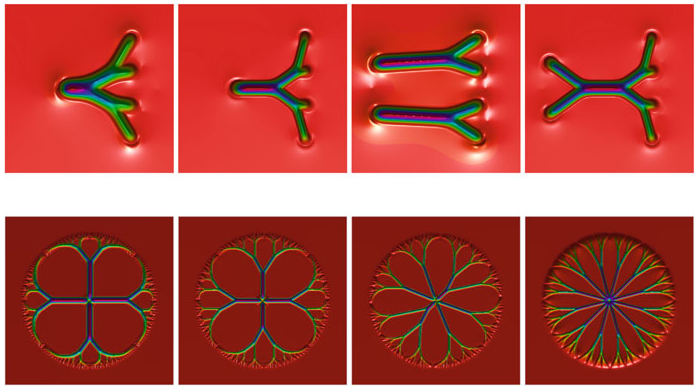
\includegraphics[width=.94\textwidth]{assets/ch04c-fig4-7.pdf}
 \caption{通过$\Gamma$收敛计算的分支运输：分别在一个点与四个点之间、两个点与四个点之间，以及一个点与圆上的均匀分布之间计算，采用不同的$\alpha$值（从左到右递增）. 部分图片经许可取自\cite{b247}.}
 \label{fig:4.7}
\end{figure}
